\documentclass[]{article}

%These tell TeX which packages to use.
\usepackage{array,epsfig}
\usepackage{amsmath}
\usepackage{amsfonts}
\usepackage{amssymb}
\usepackage{amsxtra}
\usepackage{amsthm}
\usepackage{mathrsfs}
\usepackage{color}
\usepackage{hyperref}
\usepackage[spanish, mexico]{babel}
\usepackage[utf8]{inputenc}

%Here I define some theorem styles and shortcut commands for symbols I use often
\theoremstyle{definition}
\newtheorem{defn}{Definition}
\newtheorem{thm}{Theorem}
\newtheorem{cor}{Corollary}
\newtheorem*{rmk}{Remark}
\newtheorem{lem}{Lemma}
\newtheorem*{joke}{Joke}
\newtheorem{ex}{Example}
\newtheorem*{sol}{Solution}
\newtheorem{prop}{Proposition}

\newcommand{\lra}{\longrightarrow}
\newcommand{\ra}{\rightarrow}
\newcommand{\surj}{\twoheadrightarrow}
\newcommand{\graph}{\mathrm{graph}}
\newcommand{\bb}[1]{\mathbb{#1}}
\newcommand{\Z}{\bb{Z}}
\newcommand{\Q}{\bb{Q}}
\newcommand{\R}{\bb{R}}
\newcommand{\C}{\bb{C}}
\newcommand{\N}{\bb{N}}
\newcommand{\M}{\mathbf{M}}
\newcommand{\m}{\mathbf{m}}
\newcommand{\MM}{\mathscr{M}}
\newcommand{\HH}{\mathscr{H}}
\newcommand{\Om}{\Omega}
\newcommand{\Ho}{\in\HH(\Om)}
\newcommand{\bd}{\partial}
\newcommand{\del}{\partial}
\newcommand{\bardel}{\overline\partial}
\newcommand{\textdf}[1]{\textbf{\textsf{#1}}\index{#1}}
\newcommand{\img}{\mathrm{img}}
\newcommand{\ip}[2]{\left\langle{#1},{#2}\right\rangle}
\newcommand{\inter}[1]{\mathrm{int}{#1}}
\newcommand{\exter}[1]{\mathrm{ext}{#1}}
\newcommand{\cl}[1]{\mathrm{cl}{#1}}
\newcommand{\ds}{\displaystyle}
\newcommand{\vol}{\mathrm{vol}}
\newcommand{\cnt}{\mathrm{ct}}
\newcommand{\osc}{\mathrm{osc}}
\newcommand{\LL}{\mathbf{L}}
\newcommand{\UU}{\mathbf{U}}
\newcommand{\support}{\mathrm{support}}
\newcommand{\AND}{\;\wedge\;}
\newcommand{\OR}{\;\vee\;}
\newcommand{\Oset}{\varnothing}
\newcommand{\st}{\ni}
\newcommand{\wh}{\widehat}

%Pagination stuff.
\setlength{\topmargin}{-.3 in}
\setlength{\oddsidemargin}{0in}
\setlength{\evensidemargin}{0in}
\setlength{\textheight}{9.in}
\setlength{\textwidth}{6.5in}
\setlength{\itemsep}{0.45in}
\pagestyle{empty}



\begin{document}

\begin{center}
{\huge Implementación de Modelos Computacionales TC2037-15}\\[1.5ex]
{\large \textbf{Tarea 2 -- Programación Funcional I}\\[1.5ex] %You should put your name here
} %You should write the date here.
\end{center}

\vspace{0.2 cm}

{\footnotesize \textit{En esta tarea, practicarán con Haskell para implementar múltiples funciones. Por favor consideren que el objetivo de esta tarea es permitirles practicar e identificar fuerzas y áreas de oportunidad con respecto a su capacidad. Por lo mismo, se sugiere que no utilicen funciones ya implementadas. Para facilitar cuestiones de diseño, consideren que reciben solamente argumentos del tipo de dato adecuado.}}

\section{\texttt{fibonacci} (10\%)}

Los números de Fibonacci $F$ son los números de la secuencia $0, 1, 1, 2, 3, 5, 8, 13, 21, 34, \dots$\footnote{\url{https://oeis.org/A000045}}, y tienen la peculiaridad de que cada uno se obtiene mediante la suma de los dos anteriores en la misma secuencia. Escriban una función en Haskell que reciba un número entero y devuelva el $i$-ésimo número de la secuencia, $f_i$.

\section{\texttt{evenNumbers} (10\%)}

Generen una función en Haskell que extraiga todos los números pares de una lista de enteros y los devuelva en una nueva lista.

\section{\texttt{listor} (20\%)}

Implementen una función en Haskell que recibe dos listas de enteros (1 o 0) y hace un OR lógico entre ambas entradas. Asume que las entradas son del mismo tamaño.

\section{\texttt{inverseRelation} (20\%)}

La función \texttt{inverseRelation} toma como entrada una lista de pares ordenados $(a,b)$ y devuelve la lista con los pares de la relación inversa $(b,a)$.

\section{\texttt{multiples} (20\%)}

La función \texttt{multiples} toma como entrada una lista de enteros y un número entero $x$, y devuelve aquellos números en la lista que sean múltiplos de $x$.

\section{\texttt{toBinaryString} (20\%)}

Generen una función en Haskell que reciba un número $n > 0$ y que devuelva una \textit{string} con su representación binaria.

\section*{Challenge +1 (final)}

Escriban una función que evalúe polinomios de la forma $a_n x^n + a_{n-1} x^{n-1} + \dots + a_1 x + a_0$, donde $a_i$ son los coeficientes y $x$ es la variable independiente.

\section*{Entregables}

\bigskip

\begin{minipage}{0.1\linewidth}
	\centering
	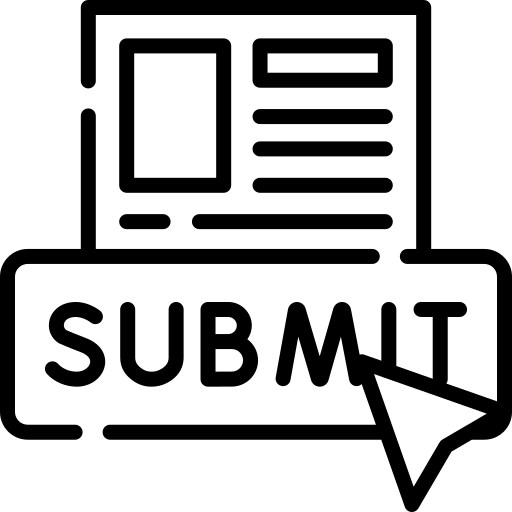
\includegraphics[scale = 0.06]{../img/submit}
\end{minipage}%
\begin{minipage}{0.85\linewidth}
	Preparen un archivo \texttt{.hs} que contenga las funciones requeridas y súbanlo a Canvas en el apartado correspondiente.
	Por favor, no suban código fuente en otro formato no editable.
\end{minipage}

\vspace{7ex}

\begin{minipage}{0.1\linewidth}
	\centering
	
\includegraphics[scale = 0.06]{../img/ribbon}
\end{minipage}%
\begin{minipage}{0.85\linewidth}
	\textbf{En esta actividad me comprometo conmigo y mi equipo a asumir un rol activo honesto y responsable, basado en la confianza y la justicia y a no servirme de medios no autorizados o ilícitos para realizarla, siguiendo el Código de Ética del Tecnológico de Monterrey}.
\end{minipage}

\end{document}